\pagebreak

\chapter{Jenkins}
Bei Jenkins handelt es sich um einen der bekanntesten Vertreter der OpenSource CI Tools. Es hat eine sehr breite Anwender Basis und dementsprechend auch viele nützliche Blogeinträge und Hands-On Berichte.
\section{Geschichte}
2004 startete Kohsuke Kawaguchi damit, Jenkins zu implementieren. Damals noch unter dem Namen "`Hudson"' und als privates Projekt. Eigentlich wollte er nur ein Tool für sich selbst entwickeln, das ihm half, qualitativ hochwertigen Code in das SCM einzufügen. (Foreword of \cite{smart2011jenkins}).\\
Das war im Jahr 2004, und er führte das Projekt neben seiner Arbeit für SUN als privates Projekt bis 2008 weiter. Zu diesem Zeitpunkt entdeckte sein Arbeitgeber das Potential dieses Tools, und er wurde gefragt, ob er nicht seine komplette Arbeitszeit für das Tool verwenden möchte, um es auf eine professionellere Ebene zu heben. Er willigte ein und bis zum Jahr 2010 erreichte Hudson einen Marktanteil von 70\%.\cite[3]{smart2011jenkins}\\
In der Zwischenzeit hatte Oracle die Firma SUN gekauft und damit auch Hudson. Ende 2010 kam es zum Zerwürfnis zwischen den OpenSource begeisterten Kernentwicklern und Oracle, in welche Richtung das Projekt ausgerichtet werden sollte. Die Meinungsverschiedenheiten, konnten nicht bewältigt werden, so dass im Januar 2011 die ursprünglichen Hudson Entwickler unter der Führung von Kohsuke Kawaguchi einen Fork bei GitHub erstellten unter dem Namen "`Jenkins"'. Auch die meisten der bisherigen Hudson Nutzer blieben dem Projekt treu und so wechselten 75\% der Hudson Nutzer zu Jenkins. \cite[3-4]{smart2011jenkins}
\section{Möglichkeiten des Betriebs}
Anfänglich war das Betreiben einer Jenkins Installation ziemlich eindeutig vorgegeben. Man musste gewisse Voraussetzungen erfüllen, wie z.B. Java und ein SCM Client und installierte dann lokal auf einem Rechner. Mittlerweile gibt es jedoch, aufgrund neuer Technologien, auch andere Ansätze, von denen ich hier drei vorstellen möchte.
\subsection{Installation direkt im Betriebssystem}
Der klassische Weg einen Jenkins CI Server zu betreiben ist die Installation direkt in ein Betriebssystem.
\begin{wrapfigure}{l}{0.5\textwidth}
  \begin{center}
    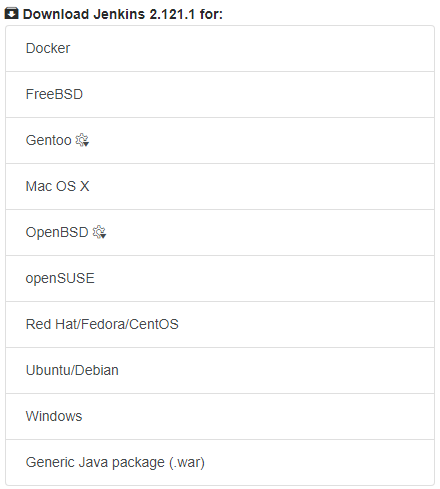
\includegraphics[width=0.48\textwidth]{./Images/Jenkins_installation_and_setup.png}
  \end{center}
  \caption{Unterstützte Betriebssystem auf der Jenkins Seite\cite{jenkins-download}}\label{Jenkins_installation_and_setup}
\end{wrapfigure}
Dazu benötigt man vor allem Java, wobei die einzige momentan unterstützte Version Java 8 ist.\cite{jenkins-java} Desweiteren mindestens 256MB RAM (1GB empfohlen) und 1GB (50GB empfohlen) Massenspeicher.\cite{jenkins-installing}
\subsubsection*{Windows}
Die Jenkins Seite bietet direkt einen Windows Installer für Jenkins an. Dieser installiert Jenkins als Windows Service, der keine Nutzer Interaktion benötigt und direkt beim Systemstart mit gestartet wird. Auch die Agents die die Builds ausführen können direkt als Windows Service gestartet werden. \cite{jenkins-windows}\\
Außerdem wird die Installation von "`UnixUtils"'\footnote{Das sind Tools die Unix-like Funktionalität nachbilden, Download unter \url{http://unxutils.sourceforge.net/} , empfohlen hier: \url{https://wiki.jenkins.io/display/JENKINS/Installing+Jenkins}} empfohlen, da Jenkins zunächst für Unix-basierte Plattformen entwickelt wurde und an machen Stellen deshalb Unix Tools voraussetzt. 
\subsubsection*{Linux}
Unter Linux kann man Jenkins ähnlich wie bei Windows als ständig laufenden Prozess installieren. Dazu erstellt man am besten einen eigenen Service Nutzer  und erstellt einen deamon um Jenkins direkt beim Systemstart zu starten. \cite{jenkins-installing}
\subsubsection*{Andere Systeme auf denen Java läuft}
Für viele andere Systeme, und als Alternative für die bereits genannten direkten Serviceinstallationen in Linux und Windows, bietet Jenkins ein generisches Java Paket an (Siehe letzte Option in \autoref{fig:Jenkins_installation_and_setup}). Diese WAR Datei kann als extra Prozess oder unterhalb eines Webcontainers wie Apache Tomcat gestartet werden \cite{jenkins-installing}
\subsection{Vorprovisionierte Container}
Das Jenkins Projekt bietet auch vorprovisionierte Container an. In \autoref{fig:Jenkins_installation_and_setup} ist der Download des Docker Containers zu sehen. Bei einem Docker Container handelt es sich um ein eigenständiges Paket, das eine Applikation und alle dazu nötigen Ressourcen enthält. Es nutzt das darunterliegende Betriebssystem um auf Systemressourcen zuzugreifen. Man kann es in etwa mit Apps auf dem Handy vergleichen.\\
Docker existiert bereits seit längerer Zeit für alle \*nix basierten Betriebssysteme, und seit Windows 10 Professional mit aktieiertem Hyper-V auch auf Windows verfügbar. Die Installation von Jenkins entfällt, man muss nur den Container starten und hat einen funktionierenden Jenkins Server.
\section{Funktionsumfang}
\section{Erweiterungsmöglichkeiten}
In den Gründen wurde AuditTrail erwähnt, hier ein Plugin dazu: \cite{jenkins-audit-trail}
